\documentclass[times,11pt]{article}
\usepackage[hmargin=1in,vmargin=1in]{geometry}
\usepackage[usenames]{color} %used for font color
\usepackage{amssymb} %maths
\usepackage{amsmath} %maths
\usepackage{graphicx}
\usepackage{hyperref}
\usepackage{xspace}

\newcommand{\GeV}{\ensuremath{\mathrm{GeV}}}
\newcommand{\TeV}{\ensuremath{\mathrm{TeV}}}
\newcommand{\GeVc}{\ensuremath{\mathrm{GeV}}}
\newcommand{\TeVc}{\ensuremath{\mathrm{TeV}}}
\newcommand{\GeVcc}{\ensuremath{\mathrm{GeV}}}
\newcommand{\TeVcc}{\ensuremath{\mathrm{TeV}}}
\newcommand{\pt}            {\ensuremath{p_{\mathrm{T}}}\xspace}
\newcommand{\kt}            {\ensuremath{k_{\mathrm{T}}}\xspace}
\newcommand{\antikt}        {anti-\kt}
\newcommand{\ttbar}        {\ensuremath{\mathrm{t}\overline{\mathrm{t}}}}
\newcommand{\bbbar}        {\ensuremath{\mathrm{b}\overline{\mathrm{b}}}}
\newcommand{\qqbar}        {\ensuremath{\mathrm{q}\overline{\mathrm{q}}}}
\newcommand{\fbinv}        {\ensuremath{\mathrm{fb}^{-1}}}
\newcommand{\instlumiA}     {\ensuremath{\times 10^{33} \,\mathrm{cm}^{-2} \mathrm{s}^{-1}}}
\newcommand{\instlumiB}     {\ensuremath{\times 10^{34} \,\mathrm{cm}^{-2} \mathrm{s}^{-1}}}

\begin{document}

\hrule
\begin{center}
{\bf \Large Clustering Jets at the Exascale}\\
Steven Ko, Salvatore Rappoccio, Lukasz Ziarek
\end{center}
\hrule
\bigskip


{\bf Overview :}
In the past, particle physics has relied upon 
improvements in processing speed of single computing cores
in order to improve data acquisition rates. This feature will be
critical to the proposed ``High Luminosity Large Hadron Collider''
(HL-LHC) and other colliders, where the computational challenges move
from the petascale to the exascale. Unfortunately, since the mid-2000's,
this improvement
in single-core processing speed has hit a limit, and
improvements in processing time must now come from concurrent
processing. However, the current reconstruction techniques are not
enabled for concurrent processing. In order to continue
improving the processing
capabilities of particle physics experiments in the HL-LHC era, it will
be necessary to explore cutting-edge techniques in parallel processing. 

There are several general classes of problems in particle physics
event reconstruction that could be modified in order to
achieve concurrent processing. One such opportunity that has not yet
been explored is in ``jet clustering,'' a nearest-neighbor type of
algorithm used to cluster hadronically-fragmented jets into a single
object. 

\bigskip
{\bf Intellectual Merit :}
This proposal focuses on parallelizing the existing jet clustering
algorithms in use at the LHC experiments. The proposed improvements
will be to use this as a test case for deployment of cutting-edge
parallelization techniques such as lightweight concurrency extraction,
speculative computing, and smarter distribution. Some recent
experience shows that the nearest-neighbor type of algorithm used by
the jet clustering is amenable to such improvements. 

\bigskip
{\bf Broader Impacts :}
The benefits of this proposal are twofold : firstly, there will be an
immediate improvement of the jet clustering algorithms themselves that
will lead to higher data acquisition rates at the LHC. Secondly, the
computing techniques developed could be used in other applications,
inside of particle physics and elsewhere. Since nearest-neighbor
algorithms are ubiquitous in scientific computing, it is expected
that techniques developed to parallelize this particular problem
will be applicable to a wide variety of others in academia and
industry. 

In addition, these core developments can train students in the newest
computing techniques, giving them cutting-edge experience that is
highly relevant in academia and private industry. 

\newpage

\hrule
\begin{center}
{\bf \Large Clustering Jets at the Exascale}\\
Steven Ko, Salvatore Rappoccio, Lukasz Ziarek
\end{center}
\hrule
\bigskip

\section{Introduction}

The research proposed here will focus on deploying advanced techniques
in parallelization to improve algorithms involved in particle physics
research at the Large Hadron Collider (LHC) and beyond. As a
specific test case, this research focuses on immediate improvements to
one particular algorithm, jet
clustering, although the principles
developed could be deployed in other areas of particle physics
reconstruction and elsewhere. 

With the discovery of the Higgs boson 
by the Large Hadron Collider (LHC)
experiments ATLAS and CMS~\cite{higgs_cms,higgs_atlas}, the
standard model (SM) of particle
physics is now complete. This model unifies the electromagnetic force
(carried by the {\em photon}) with the weak force, responsible for
radioactive decay (carried by the {\em $W$ and $Z$ bosons}).
At long last,
physicists now understand that via interactions with the Higgs field,
the $W$ and $Z$ bosons acquire a mass, but the photon does not. 
This is referred to as ``electroweak symmetry breaking''. 


A new phase of particle physics has therefore begun. 
The questions have shifted from the cause of electroweak symmetry
breaking, to the study of the Higgs boson and its interactions in
detail. To understand the larger picture of the fundamental forces in
nature, it will be imperative that high-luminosity colliders be built
to study the Higgs in detail, requiring exascale computing tools (in
speed and throughput) to reach the goals. 


One of the major technical challenges that lies ahead in
exascale-level computing for these high-luminosity colliders is the
continuation of the scaling of computational power year by year, known
colloquially as ``Moore's Law''. 
To set the scale, at the CMS experiment
with the LHC collision flux (``luminosity'') reaching
$7\instlumiA$, the processing
time to reconstruct each collision event by CMS was approximately 20
seconds per event. However, as the luminosity is
increased, the computational time currently scales
quadratically. The luminosity at the HL-LHC is expected to reach as
high as $>1\instlumiB$, which would correspond (naively) to enormous
processing times, on the order of many minutes to several
hours per event! Clearly, it is necessary for the
computing power to scale in order to compensate for this dramatic
increase in CPU time with increasing luminosity. 

Unfortunately, the expected end of the historic scaling of single-core
processing capability~\cite{GAMEOVER} can adversely affect the
long-term processing capability for particle physics
experiments. Without improvements in single-core computational speed,
the only avenues left are algorithmic improvements, and
parallelization. Algorithm development is being undertaken at the LHC
experiments to
reduce the computational time of the software for data acquisition and
reconstruction, using both single-core and multi-core
approaches. However, long-term improvements will require fundamental
improvements in processing capabilities using parallelization. 

The currently proposed exploratory research will deploy new and
innovative computer science techniques to particle physics. 
One algorithm that is particularly amenable to improvement using these
techniques is the clustering of
final-state particles produced in collisions into groups called
``jets''. Jets are produced via quantum chromodynamic (QCD)
interactions of quarks and gluons that hadronize. 
These ``jet clustering'' algorithms group the particles into jets
based on nearest-neighbor clustering (NN). 
This algorithm can become computationally expensive as the number
of particles that are produced in a collision grows, scaling as
$N^2\log{N}$ or $N\log{N}$. Techniques that leverage and combine speculative computing,
lightweight concurrency, and smarter distribution can strongly impact
these types of NN algorithms~\cite{knn_gpu_1,knn_gpu_2,knn_gpu_3,knn-mapreduce-0,knn-mapreduce-1}. 
Thus, this research will serve as a real-world test case
for the deployment of these algorithms, with both immediate and
long-term benefits. 



%At CMS, this computation is done very often by individuals rather than
%centrally, and so is accounted for
%in the 40\% of CPU usage from ``mixed user analysis applications'' as
%described above. 
%It is likely, therefore, that improvements observed
%in jet clustering will primarily benefit this portion of the CPU
%usage. 
%We now discuss the prospects for
%utilizing parallelization in jet clustering in detail. 

 
\section{Prior Work}


\subsection{Results from Prior Support}

All three PIs are junior faculty members at the University at Buffalo. 
PI Rappoccio and Co-PI Ziarek joined the faculty in their
respective departments in August 2012.

\subsubsection{PI Rappoccio}
PI Rappoccio does not have NSF support yet as he has recently started his
faculty career.

\subsubsection{Co-PI Ziarek}
Co-PI Ziarek does not have NSF support yet as he has recently started his
faculty career.

\subsubsection{Co-PI Ko}
Co-PI Ko has been awarded ``CI-ADDO-NEW: PhoneLab: A Programmable Participatory
Smartphone Testbed'' on 06/01/12. The award number is CNS-1205656 and the amount
is \$1,358,510.00. The duration is for three years. The results include the
following.

\paragraph{Results Related to Intellectual Merit:} the PhoneLab team has
distributed 300 smartphones to the faculty, students, and staff of UB who are
using the smartphones as their primary phone. The team has developed the testbed
infrastructure where they can monitor the usage of each phone. The team has also
developed a front-end website where experimenters and participants can use for
various testbed-related functions. The team has opened the PhoneLab testbed for
public experimentation on 10/31/13. There are two public experiments running on
the testbed and 7 experiments are waiting for approval.

\paragraph{Results Related to Broader Impact:} the PhoneLab team is in the
process of recruiting 4 undergraduate students as part of their outreach
program. Two undergraduate students have been working with the team for one
month now. The team is actively interviewing undergraduate students to hire. In
addition, the team is in talks with Buffalo Academy of Science Charter School in
order to explore the possibility of establishing a program where the team
teaches high school students with smartphone programming skills.

\paragraph{Publications:} the PhoneLab team has published one paper so far,
``PhoneLab: A Large Programmable Smartphone Testbed'' in the First International
Workshop on Sensing and Big Data Mining, 2013.

\paragraph{Evidence of Research Products:} the PhoneLab testbed is currently in
use; there are roughly 300 participants and several experiments are either
running or waiting for approval. Experimenters can submit their experiments
through the website: \url{http://www.phone-lab.org}.

\subsection{Overview of Activities}

The investigators of this proposal have a
widely-varied and applicable skill set to accomplish the goals of
extending LHC computing to the exascale. 



%\bigskip
%\noindent
%{\bf Particle Physics Computing}
%\bigskip

Salvatore Rappoccio (tenure-track Assistant Professor) joined the
Faculty at the University at Buffalo, SUNY (UB) in 2012. He has 15
years of experience programming in a
high-energy physics environment, as well as other numerical software
design for the private sector.

Since 2007, Rappoccio has been a member of the Compact Muon Solenoid
(CMS) experiment at CERN. 
From 2008-2010, he was the co-leader of the Analysis Tools group of
the CMS Software Project. He was responsible for deployment of jet
reconstruction algorithms as well as other tools for data analysis of
LHC collision data during the startup phase of the LHC. His primary
responsibilities included managing deployment of highly-performing
software (including visualization) tools in a team consisting of
$\sim$15 people. He has been instrumental in improving the single-core
computational speed for jet clustering at CMS since 2008. 

His research interests include utilizing jet clustering algorithms in
new and innovative ways to search for signals of physics beyond the
standard model of particle physics. His pioneering efforts resulted in
the first measurements and searches for new phenomena with advanced jet clustering
algorithms at CMS, outlined in 
Refs.~\cite{EXO-11-006,EXO-11-095,SMP-12-019}. These
techniques have become hugely popular in the LHC experiments and in
the theoretical community. Prof. Rappoccio is a leader in the jet
reconstruction community, contributing to and editing seminal reports
on the subject in Refs.~\cite{boost2010,boost2011,boost2012}.
In addition to this academic work, he has also been involved in
numerical software design for MIT's Lincoln Laboratories (the details
of which are classified). 

Currently, Rappoccio is mentoring two students (one graduate student,
Jaba Chelidze, and one undergraduate student, Jonathan Goodrum) in
achieving parallelization of the jet clustering algorithms. The latter
is working under the ``Collegiate Science and Technology Entry
Program'' (CSTEP)~\cite{cstep}. As described by the program, CSTEP
exists ``to support talented underrepresented students pursuing
science, technology, engineering and mathematics''. 


Lukasz Ziarek has 9 years of experience in language, compiler,
and runtime design targeted at improving multicore performance.  He
has worked on 5 compilers and 3 Java VMs. He is an expert at
speculative and transactional computation focusing on the extraction
of parallelism and lightweight concurrency. 



Steven Ko has 10 years of experience in distributed systems. His
recent focus has been large-scale data processing in the cloud using
MapReduce and other technologies built on top of it. He also has 5
years of experience in large-scale storage and data management in
data centers.


\section{Proposed Program of Research}


The
``jet clustering'' technique is employed by
many different particle physics experiments and theorists worldwide, and is
implemented in a common software framework called 
{\tt fastjet}~\cite{fastjet_manual}. 
The mathematical problem is analogous to the
``K-nearest neighbors algorithm''~\cite{knn_ieee} (kNN). 


The specific jet-clustering algorithms that have become enormously
popular in the particle physics community are based on sequential
clustering, similar to nearest-neighbor
clustering~\cite{fastjet_timing}. In these sequential-clustering
algorithms, a list of the four-momentum of particles are input. 
These algorithms combine the input four-vectors pairwise
until certain criteria are satisfied, defining the resultant
combination as a jet. 
For the jet algorithms considered in this proposal, for each pair of particles $i$ and $j$,
a ``distance'' metric between
the two particles ($d_{ij}$), and the so-called ``beam distance''
for each particle ($d_{iB}$), are computed:



\begin{eqnarray}
\label{eq:dij}
d_{ij} &=& \mathrm{min}({\pt}_i^{2n},{\pt}_j^{2n}) \Delta R_{ij}^2 / R^2 \\
\label{eq:diB}
d_{iB} &=& {\pt}_i^{2n}, 
\end{eqnarray}

where ${\pt}_i$ and ${\pt}_j$ are the transverse momenta of particles
$i$ and $j$, respectively, ``min'' refers
to the lesser of the two $\pt$ values, 
the integer $n$ depends on the specific jet algorithm, $\Delta R_{ij} = \sqrt{(\Delta y_{ij})^2 + (\Delta\phi_{ij})^2 }$
is the distance between $i$ and $j$ in
rapidity ($y = \frac{1}{2} \ln (E + p_{z})/(E - p_{z})$) and azimuth ($\phi$),
and $R$ is the ``size'' parameter of order unity~\cite{ktalg}, with all angles expressed in radians. 
The particle pair $(i,j)$ with smallest $d_{ij}$ is combined into a
single object. All distances are recalculated using the new object, and the procedure is
repeated until, for a given object $i$, all the $d_{ij}$ are greater
than $d_{iB}$. Object $i$ is then
classified as a jet and not considered further in the algorithm. The process is
repeated until all input particles are clustered into jets. 


The value for $n$ in Eqs.~(\ref{eq:dij}) and~(\ref{eq:diB}) governs
the topological properties of the jets. 
For $n=1$ the procedure is referred to as the
$k_{\mathrm{T}}$ algorithm (KT). The KT jets tend to have irregular
shapes and are especially useful for reconstructing jets of lower momentum~\cite{ktalg}.
%For this reason, they are also sensitive to the presence of 
%low-$\pt$ pileup (PU) contributions, and are  
%used to compute the median $\pt$ per unit area (in $(y,\phi)$) of an
%event~\cite{jetarea_fastjet}. 
For $n=-1$, the procedure
is called the anti-$k_{\mathrm{T}}$ (AK) algorithm, with features
close to an idealized cone algorithm. 
%% when the input particles have
%% negligible mass, in which case the rapidity $y$ is approximated by the
%% pseudorapidity $\eta$. 
The AK algorithm is used extensively
in LHC experiments and by the theoretical community for
finding well-separated jets~\cite{ktalg}. For $n=0$, the procedure
is called the Cambridge--Aachen (CA) algorithm. This relies only on angular
information, and, like the $k_\mathrm{T}$ algorithm,
provides irregularly-shaped jets in $(y,\phi)$. The CA algorithm is useful in identifying
jet substructure~\cite{CAcambridge,CAaachen}.




The single-core optimization of
jet clustering
is outlined in Ref.~\cite{fastjet_timing}. In a single core,
the computational time scales as $O(N^2)$ or  $O(N \ln{N})$, where $N$
is the number of inputs to the algorithm, which scales linearly with
luminosity. Since the luminosity of future colliders is expected to
drastically increase over existing machines, it will be critical to
develop parallelization strategies to maintain scalability of the jet
clustering algorithms that exist to future machines. 

Since the particles are clustered pairwise, there are numerous
opportunities to separately compute portions of the event and then
combine them at later stages. 
We now
discuss specific strategies that can be developed 
to optimize concurrent performance in this algorithm. 


\iffalse
There is existing work and literature on the topic of the
parallelization of similar kNN algorithms, for instance, in
Refs.~\cite{knn_gpu_1, knn_gpu_2, knn_gpu_3}, where improvements
$O(100)$ in CPU performance are observed over standard
algorithms. Since the proposed use case is
very similar to the kNN algorithm, similar improvements to the
processing time by parallelization strategies are expected. 
\fi



\subsection{Technical Challenges}

To achieve the necessary improvements in performance required for scalability
of jet clustering, we propose to examine parallelization opportunities across
the entire software stack, including three specific areas : 
(1) the use of lightweight concurrency
extraction to mask high-latency computations or I/O actions, 
(2) extraction of
parallelization from the computation itself in the form of optimistic speculation
and specialized transform, and
(3) new methods for distributing the computation to
maximize parallelization on each node. 


\bigskip
\noindent
{\bf  Lightweight Concurrency for Latency Masking}
\bigskip

Many mathematical kernels contain opportunities for extracting ``micro parallelism,''
usually on the order of tens of instructions, from their computational components. 
Unfortunately, it is very difficult to parallelize this computation profitably as
the overhead of thread creation, scheduling, synchronization, and migration outweigh
the gains in parallelism. Instead of extracting explicit parallelism from such
computations, we propose to explore methods of lightweight asynchrony to allow for
computation to proceed while waiting on high latency I/O operations to complete or on
the results of other computations. Since the creation of threads and associated
schedule and synchronization costs are typically prohibitive, we will explore new
threading models that allow for logically-distinct computations to execute within
a given construct. Co-PI Ziarek's previous research has indicated that such schemes can profitably
boost overall performance in the context of ML code~\cite{acml, parasites}. 
The salient research
challenges in applying this strategy are as follows:  1) identifying what computation can be executed
safely during high latency operations at compile time, 2) providing a lightweight threading runtime
and programming model in the context of an imperative language, 
3) specializing the approach to numeric kernels,
and 4) building support for computation in a distributed setting.

\bigskip
\noindent
{\bf Speculative Computation}
\bigskip

In addition to exploring explicit parallelization of the numeric kernels in jet clustering, we
propose to explore extraction of parallelism via speculative computation. At its core, speculative
computation breaks apart sequential or parallel tasks into smaller tasks to be run in parallel. Once
the speculation has completed, the runtime system validates the computation. If the computation is
incorrect ({\em i.e.} a ``datarace'' is detected, the computation cannot be serialized, {\em etc.}), the
incorrect computation is re-executed in a non-speculative manner.  If the rate of mis-speculation
is low, such techniques can be leveraged to extract additional
parallelism. 
There have been many different
proposals, including large efforts on transactional memory~\cite{Gramoli:2012:TCS:2168836.2168872,Bocchino:2008:STM:1345206.1345242,Adl-Tabatabai:2006:CRS:1133981.1133985,Usui:2010:ALC:1850844.1850945},
lock elision~\cite{Roy:2009:RSS:1519065.1519094}, thread level speculation and speculative
multithreading~\cite{Barreto:2012:UTS:2442626.2442639,Johnson:2004:MPD:996841.996851},
 for integrating speculative computation into programming languages
 and their associated runtimes.
The PIs have extensive experience with transactional memory~\cite{trans}, lightweight rollback methods~\cite{stab}, 
leveraging memoization to reduce re-computation costs~\cite{memo1, memo2},
and deterministic speculation~\cite{iso}. We propose to explore a specialized speculation framework leveraging different
speculation strategies, including speculation extracted by the programmer via programming language primitives,
library level speculation, and compiler extracted speculation.
The salient research
challenges in applying this strategy are as follows:  1)
identification of the appropriate speculation model and
discovering speculation points at compile time, 2) providing a speculative runtime specialized for jet clustering
and capable of realizing user, library, and compiler injected speculation, and 3) exploring new and specialized
lightweight validation and re-execution mechanisms, including validation across multiple speculation strategies.



\bigskip
\noindent
{\bf Smart Distribution}
\bigskip

In order to increase parallelism, we will explore the use of the MapReduce
execution framework~\cite{mapreduce-osdi, mapreduce-hadoop}. MapReduce is a
runtime system recently developed for large-scale parallel data processing. It
enables programmers to easily deploy their applications on a cluster of
machines. Programmers only need to write two functions, Map and Reduce, and
submit these two functions as a job to the system. Then the MapReduce framework
takes care of all the aspects of the execution of the job. For example, the
framework packages and distributes the two functions over the cluster so that
the whole cluster can be utilized to execute the job; it also takes care of
fault-tolerance by monitoring the cluster during the execution of the job and
redistributes the job if some machine fails.

Due to this simplicity and power, it is quickly gaining popularity in industry
for large-scale data processing. Many applications in scientific computing have not
yet explored the use of MapReduce in depth, however
previous research has explored implementing similar kNN-style
algorithms with
MapReduce~\cite{knn-mapreduce-0, knn-mapreduce-1}. We intend to explore this
question in the context of jet clustering for the LHC.



\subsection{Research Strategy}

Preliminary studies of naive parallelization of a few specific
routines in the {\tt fastjet} package reduced processing times by
factors of 2-3 by moving to concurrent processing with 8 cores, with
no increase in memory cost. By further deploying the advanced
strategies described above, this factor of 2-3 improvement is expected
to grow significantly. 
These preliminary studies were performed by Rappoccio and Mr.
Goodrum (undergrad student) over the summer of 2013. Having a
postdoctoral fellow to work on this project will greatly increase the
likelihood of success. 

The postdoctoral fellow requested in this proposal is envisioned to
have a computer science background. There will be two graduate
students, one with a physics background (but with strong computational
skills), and one with a computer science background. Furthermore, it
is expected that Mr. Goodrum will continue to work with the group
under his CSTEP Fellowship. This team, under
the guidance of Rappoccio, Ziarek, and Ko, will perform the
implementation and study of these algorithms in the real-world 
{\tt fastjet} software environment, testing the improvements at the
extensive cluster at the {\bf Center for Computational Research} here
at UB. 

During the first year, it is expected that naive improvements using
established techniques could be deployed into the {\tt fastjet}
package. Deployment of the improvements achieved by Mr. Goodrum and
Rappoccio should take several months to a year of full deployment
time. This will serve as a baseline for the advanced algorithmic
improvements that will be in research and development simultaneously. 

The postdoctoral fellow, under the tutelage of Profs. Ziarek, Ko, and
Rappoccio, will use this baseline to investigate the impacts of speculative
computation and lightweight concurrency. In the first half of the first year,
we will first start with the task of exploring lightweight concurrency
techniques as this is applicable in multiple settings, including single machines
and clusters. Two graduate students will contribute to
this effort. During this period, they will gain more experience with the kNN
algorithm and also with the existing code base.

Starting from the second half of the first year, the PIs and the postdoctoral
fellow will move on to the task of investigating speculative computation, while
two graduate students finalize and polish the implementation of lightweight
concurrency techniques. Due to the number of options we can investigate and the
complexity of the implementation of the techniques, we anticipate that this task
will be more involved in terms of the initial investigation and overall
development. Thus, we will start this task from the second half of the first
year and continue throughout the second year. Based on prior results of
the PIs and the community, we expect to gain scalability increases of
2x to 8x over the naive parallel algorithm with these techniques. Additional
improvement in throughput is expected by masking high latency I/O operations and network
communication. 

We will spend the final year mostly with smart distribution strategies and
integration of the techniques we develop in the first two years. Due to its
unique programming model, MapReduce brings its own complexity and the
postdoctoral fellow and the two graduate students will spend the beginning of
the third year to learn how to program in MapReduce. After that, we will
investigate how to adapt our kNN algorithm with MapReduce. Table~\ref{timeline}
shows the proposed project timeline. We expect to get additional overall
system throughput for the kNN algorithm and improved scalability. Based on
prior results we expect to see improvements of 2x to 4x.  Additional
improvements can be expected as the cluster size increases.

\begin{figure*}[!tp]
\centering
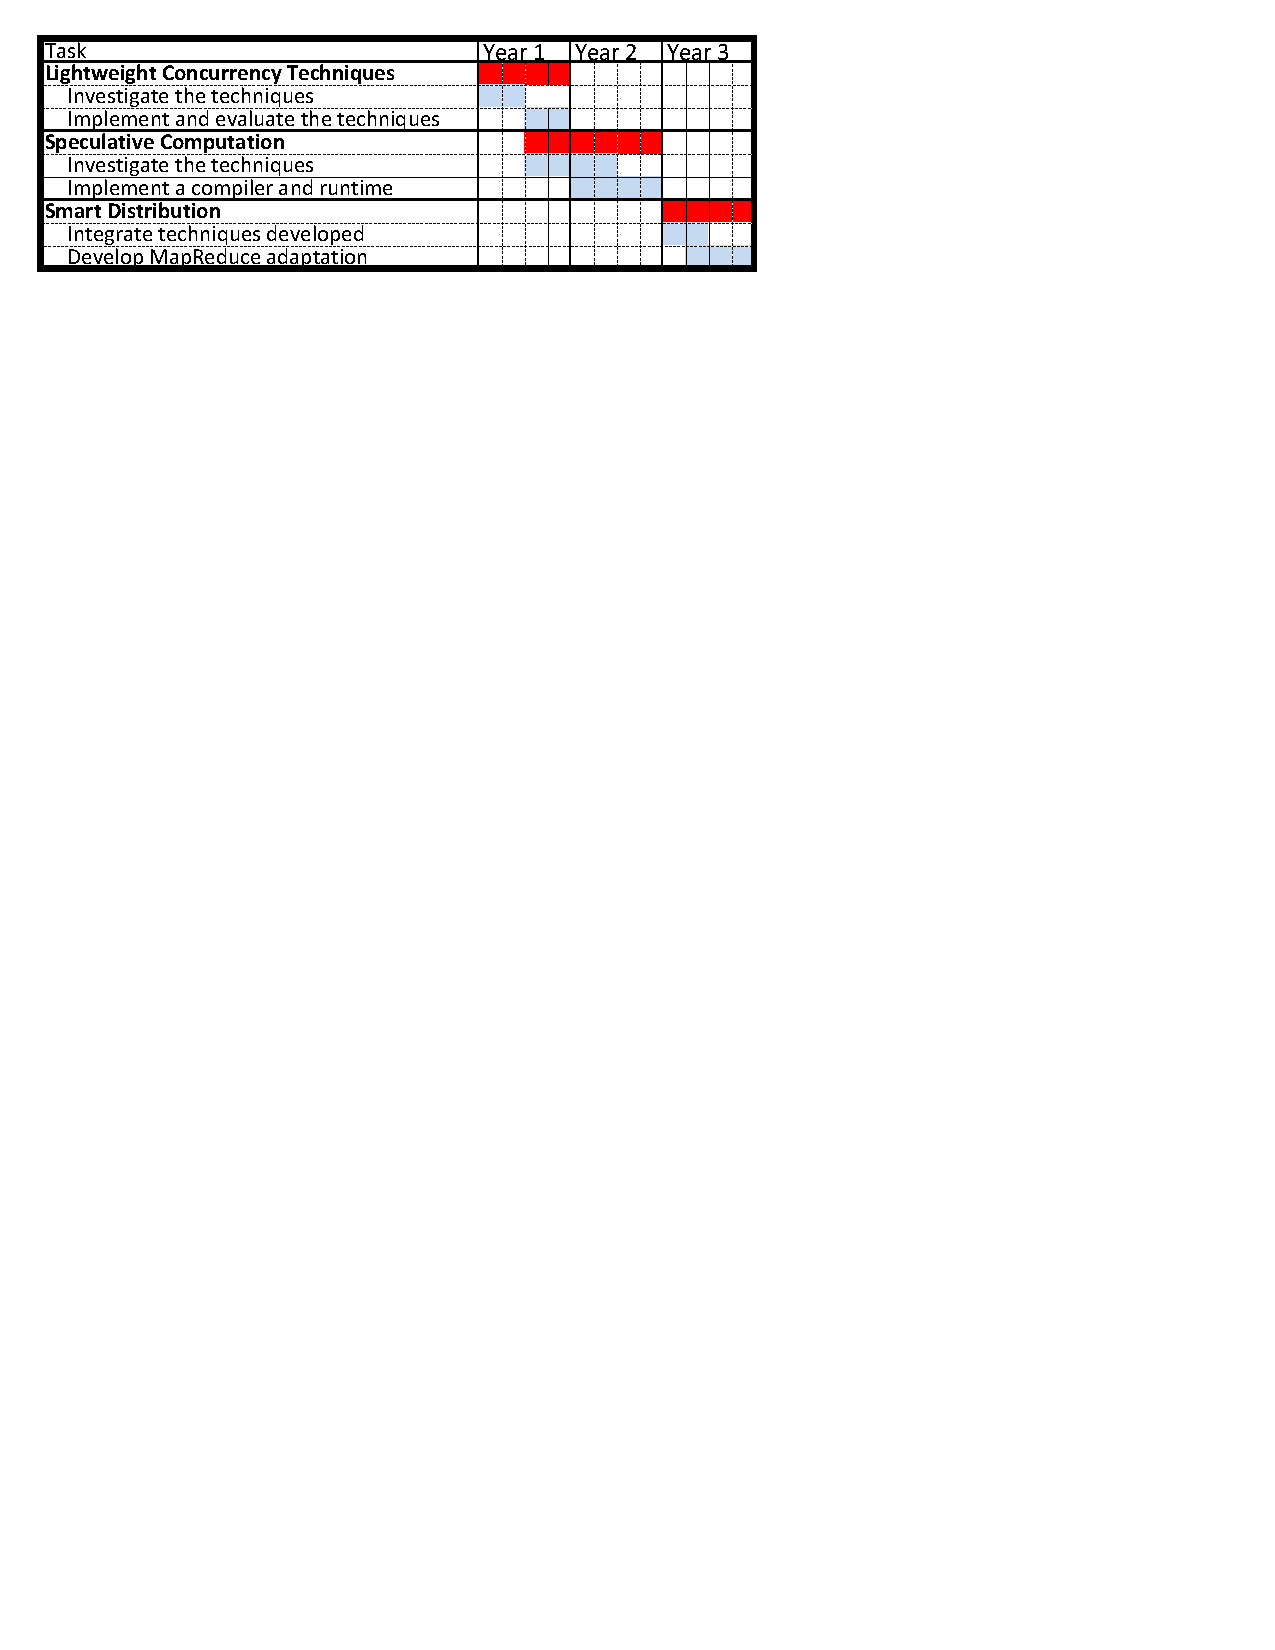
\includegraphics[width=0.80\textwidth]{schedule.pdf}
\caption{Project Timeline}
\label{timeline}
\end{figure*}

\section{Broader impacts}

The broader impacts of this research are manyfold. The jet-clustering
algorithm is very similar to the ``kNN'' algorithm, which is widely
applicable throughout research and industry. The improvements that are
developed here at the cutting edge of scientific inquiry will possibly be
adaptable to other real-life applications. Examples of applications
outside of particle physics would be statistical
software~\cite{statsoft}, real-time 3-d rendering of computer
graphics~\cite{opengl}, and feature extraction~\cite{featureextract}. 

In addition to the core physics developments enabled by improved
scalability of the {\tt fastjet} software environment, this award will
also serve as a validation mechanism for core computer science
research in programming languages and distributed systems.  The development
of the system will require systems research in expanding and applying
the technological advances made previously by the PIs.



\section{Education and Outreach}


\subsection{Education}
All three PIs teach graduate courses at UB and will teach undergraduate courses
during the duration of this project.  In this section we outline planned activities
and how they relate to the proposal.


\subsubsection{Curriculum Development}

{\bf Undergraduate (UG) level.}
Co-PI Ko teaches undergraduate {\bf Networking} and {\bf Systems} courses. Co-PI Ziarek will
teach undergraduate {\bf Compilers} and {\bf Programming Languages}
courses. 
PI Rappoccio teaches undergraduate 
{\bf Introductory Computational Physics} and {\bf Introductory Physics}. 
All three PIs plan on creating a cross-listed Physics/Computer Science course
focusing on advanced and modern techniques in scientific computing
beyond the traditional computational physics classes. The courses will be geared toward
advanced undergraduates and graduates in Physics and Computer Science.
Software developed under this proposal will be leveraged in the
classroom to exemplify practical aspects of the work.


{\bf Graduate (G) level.}  
Co-PI Ko teaches graduate {\bf Distributed Systems} and {\bf Android} courses. Co-PI Ziarek will
teach graduate {\bf Programming Languages} courses. PI Rappoccio
teaches a graduate version of {\bf Introductory Computational Physics}. 
The PIs plan on teaching a graduate version
of their proposed undergraduate course, focusing on advanced techniques and implementation
details at the systems level.  Students who successfully complete the course will be well suited to
begin research at the intersection of particle physics and computer science. To help support
students interested in this advanced course, two three week winter session courses will be offered: 
one for computer science students to teach the necessary physics background and one for physics
students to teach systems and distributed programming.  The proposed course will be taught
in the spring semester after the winter session courses.

\subsubsection{Undergraduate research and Diversity}

PI Rappoccio works closely with
undergraduates, including Mr. Goodrum. Mr. Goodrum is participating in the
``Collegiate Science and Technology Entry Program'' (CSTEP) here at
UB while working on this project. This program focuses on
disadvantaged or minority students who would otherwise have a
difficult time pursuing STEM-related fields. Prof. Rappoccio is a
strong believer in the principles and practice of this program, and
intends to continue this work in the future. 
There are also numerous opportunities for Independent Study and
Honors' Theses for undergraduates in the Physics department. 

Co-PI Ko is actively involved in mentoring undergraduates. Co-PI Ko is involved
in several formal programs such as the McNair Program and UB Honors College
Program. Through these programs, two undergraduate students, Edward Poon and
Mitchell Nguyen, are currently conducting research with him. Edward Poon, a
junior, participates in the McNair Program, which is ``designed to provide
encouragement and services to low-income and first generation college students,
and increase participation from underrepresented groups in pursuing doctoral
study.''~\footnote{\url{http://cads.buffalo.edu/mcnair}} Co-PI Ko is currently
listed as a McNair mentor. The other student, Mitchell Nguyen, is a freshman
Honors College student. Mitch was involved in Co-PI Ko's research and
hopes to continue his research involvement.

Co-PI Ko also has a track record of recruiting women students. Co-PI Ko has
successfully recruited two female PhD students, Sonali Batra and Anudipa
Maiti. Co-PIs Ko and Ziarek have also been working with a female Master's
student, Namita Vishnubhotla, and have successfully recruited her as a PhD
student; she will start as a PhD student in Spring, 2014. All PIs will
actively continue to recruit female and minority students in their research
programs.

\subsection{Outreach}

While it is critical to pursue a rigorous research program, a large
part of the responsibility of scientists is to educate the next
generation effectively. There is already extensive work being done to
educate high school-level students and teachers about particle physics
via the {\em QuarkNet}
program  at UB, however there is
very little in the way of educating the general
public. 
In addition to participating in the existing {\em QuarkNet}
activities, the plan outlined in this proposal will extend the coverage of the
outreach program at UB to engage the broader
public in discussions of major results in particle
physics, as well as to enliven particle physics for young students. 
This will be implemented based on similar events as the
``HiggsFest''~\cite{higgsfest} that PI Rappoccio organized at UB. 
In addition, outreach directly to high school environments will be
undertaken based on the Computer Science Teachers Association (CSTA)
work done by Co-PI Ziarek. 


\subsubsection{Higgsfest and other public events}

The ``Higgsfest'' that was organized here at UB in 2012
is highlighted in Ref.~\cite{higgsfest}. The aim of the event was to
invite the general public for ``plain English'' summaries and hands-on
demonstrations that were geared for a multitude of age and knowledge
levels. 
This was attended by over 100 people, including children,
high-school students, physics and non-physics undergraduates, and
interested members of the community. 

Some of the hands-on demonstrations included building models of
Feynman diagrams from craft material (for young children), a
fully-functional four-layer coincidental muon scintillator detector,
a cloud chamber made out of tupperware, felt, and dry ice, and the
actual Higgs events from the CMS collaboration in an interactive event
display. 
The event was covered by the ``UB Reporter'' here at
UB~\cite{higgsfest_ubreporter}. 

Two more such events are proposed, the first to coincide with the LHC
turn-on sometime in 2015, and the second to coincide with the newest
results from the LHC after data-taking commences. These are 
events that should generate high media coverage, and will be a good
opportunity to capitalize on public interest in this field.
In the event of a major new discovery at the LHC
during Run 2, the public interest will be very high, so having the
experience of what works and what does not work in such events is
extremely valuable to maximize the public impact. 

In addition, this removes the stigma associated with science and
technology fields at an early age. When young children can attend an
event with their parents and take something away from it, this shows
them that science is an integral part of life, and nothing to be
particularly nervous about pursuing. It may even convince younger
people to pursue a scientific career. 

One of the major points learned during the last ``Higgsfest''
is that it is often difficult to have economically-disadvantaged
students attend the lectures because of a lack of transportation
possibilities. This is something to rectify for future
projects along these lines. Therefore, in addition to holding the
event directly
at the UB North Campus (which is difficult for inner-city
Buffalo schools to reach), a duplicated event is also proposed
closer to the inner city that is easier to attend, or possibly to
visit these schools directly. Some possible
locations are the UB South Campus, or at
``Babeville''~\cite{babeville}, where the UB Physics
Department routinely organizes the ``Science and Art
Cabaret''~\cite{cabaret}. Both locations 
provide the infrastructure needed for the event, and
access for disadvantaged schools and students in the inner city of
Buffalo. 

\subsubsection{High School Outreach}
Co-PI~Ziarek is heavily involved with the local and national chapters of the Computer Science Teachers Association (CSTA), which
focus on outreach to local high school teachers. He has helped organize the annual local conference for high school teachers in
2012 and 2013, he has developed and presented a half day Python workshop that shows teachers how to leverage Python and
robotics in the classroom, and has been an invited speaker at the CS4HS program offered at Buffalo State University.
PI~Ziarek expects to continue to offer
material for use at the high school level and plans to teach an age appropriate  workshop on scientific computing at the next
CSTA conference. One goal of the CSTA is to attract underrepresented minorities to study computer science through
exposure and education at the high school level.  
The PIs expects to leverage the software developed under this proposal to offer age appropriate material to HS teachers 
through the use of a Python interface. Specifically,
introductory programming modules along with associated lessons plans to integrate either individual units or entire
curriculums into the classroom.


\section{Summary}

In summary, the problem of expanding LHC computing to the exascale is
a difficult, but tractable one. This proposal investigates the
possibility of applying cutting-edge parallelization techniques such
as lightweight concurrency extraction, speculative computation, and
smarter distribution, to the
real-world application of LHC data processing.
The overall goal is to reduce the computational time for
$k$-nearest-neighbor-like numerical kernels used for jet
clustering. The investigators of this
proposal have extensive experience in the various aspects of the
problem, and the synergistic application of this experience is
expected to attain considerable improvements in this area, which
are absolutely critical to the success of the future LHC physics
program. 



\newpage
\pagenumbering{arabic}
\renewcommand{\thepage} {A--\arabic{page}}


\bibliographystyle{unsrt}
\bibliography{NSF-PIF2013}{}
%\bibliography{auto_generated}

\newpage
\pagenumbering{arabic}
\renewcommand{\thepage} {B--\arabic{page}}
\noindent{\Large \bf BUDGET JUSTIFICATION}

\bigskip
{\bf Institution : } The State University of New York at Buffalo (UB)

{\bf PI : } Salvatore Rappoccio

{\bf Co-I : } Lukasz Ziarek, Steven Ko


\bigskip
{\bf Personnel}
\bigskip


The requested funds of \$951,102 USD (for 3 years starting in 2014)
would cover two (2) months of summer salary for Profs. Rappoccio,
Ziarek and Ko per
year for three (3) years
(\$172,062), the full salary for 
one (1) postdoctoral fellow for three (3)
years (\$154,224), and salary plus
tuition for two (2) graduate students, totaling \$91,812 in
salary and \$33,432 in tuition. This will also cover \$22,300 of
computer fees. 

If awarded, efforts for Profs. Rappoccio, Ziarek and Ko will be
reduced to be in compliance with NSF 2 month policy. 

\bigskip
{\bf Fringe}
\bigskip


Fringe benefit rates are based on the applicable federally negotiated rates published at
\\
http://www.research.buffalo.edu/sps/about/rates.cfm.


\bigskip
{\bf Travel}
\bigskip

This research will require regular travel to conferences and
CERN. Hence, the proposal requests
\$12,486 in domestic travel funds and \$12,486 in foreign travel funds
for the three years of activity. 

\bigskip
{\bf Facilities and Administration Indirect Costs}
\bigskip

Indirect cost rates are based on the applicable federally negotiated
rates published at 
\\
http://www.research.buffalo.edu/sps/about/rates.cfm





\newpage
\pagenumbering{arabic}
\renewcommand{\thepage} {C--\arabic{page}}
\noindent{\Large \bf Facilities, Equipment and Other Resources}


\bigskip
{\bf Center For Computational Research}

UB has a large computational research center, CCR, which is a
Linux-based cluster on the Open Science Grid, and also has a large GPU
cluster for possible parallel processing developments. 

\bigskip
{\bf Office}

The faculty, postdoctoral fellows and graduate students all have
office space at UB. 


\newpage
\pagenumbering{arabic}
\renewcommand{\thepage} {D--\arabic{page}}
\noindent{\Large \bf Postdoctoral Fellow Mentoring}

One postdoctoral fellow will be funded on this project. There are
extensive postdoctoral fellowship mentoring activities at UB, as well
as via the CMS
Experiment at CERN. These include guidance in career paths,
work/life balance discussions, and technical skill development such as
writing grant proposals, etc. Specific elements are highlighted
below. 

\begin{itemize}
\item {\bf University at Buffalo (UB)}
\begin{itemize}
\item The UB Office of Postdoctoral Scholars offers diverse services
  for postdoctoral fellows, including the {\sl ``Postdoc Survival
    Skills Workshops''}, targeted seminars and symposia for
  postdoctoral fellows, social functions, and logistical assistance. 
\item The UB Physics Department offers several services to our
  postdoctoral fellows, including a biweekly Journal Club for particle
  physics and cosmology, weekly seminars and colloquia, and weekly
  social functions inside the department. 
\end{itemize}
\item {\bf CERN}
\begin{itemize}
\item The opportunities for a postdoctoral fellow at CERN
  are extensive. There are also a plethora of workshops,
  seminars, conferences, etc, at CERN. There are also smaller weekly
  avenues for networking possibilities, as well as seminars for
  postdoctoral fellows to gain visibility for their work. 
\item It is also worth pointing out that, because of the world-class
  nature of CERN, it often attracts very high-level members of the
  particle physics community on a regular basis. Such opportunities
  for visibility among the top-tier scientists in the world (including
  Nobel and Milner Prize winners, etc) are hard to understate. 
\end{itemize}
\end{itemize}

In all, the postdoctoral fellow that will be supported by this
proposal will have ample opportunities for professional advancement
and development, as well as a myriad of opportunities for a community
of peers in both professional and social settings. 



\newpage
\pagenumbering{arabic}
\renewcommand{\thepage} {E--\arabic{page}}
\noindent{\Large \bf Data Management Plan }



The data that are produced from this proposal will be in the form of
software algorithms and procedures. The format and content will be as
source files (typically {\tt C++}). There will be no data nor metadata
collected. 

The algorithms that are developed with this research plan will be
integrated into the main {\tt fastjet} software framework for
distribution among collaborators (both experimental and theoretical)
worldwide (\url{http://fastjet.fr}). This software is open-source,
freely available, and continually maintained by the {\tt fastjet}
maintenance team under the GNU Public License V2~\cite{gnupl}. 
The web pages related to this project are stored on
machines at the ``Laboratoire de Physique Théorique et Hautes Energies'' 
(\url{http://www.lpthe.jussieu.fr/spip/?lang=en}). 

The {\tt fastjet} team has indicated their willingness to integrate
improvements into the main {\tt fastjet} package for worldwide
distribution. 





\end{document}

% LocalWords:  Exascale LHC Ko Rappoccio Lukasz Zialek Ziarek EIC PIs
% LocalWords:  Collider exascale transformative CMS multicore VMs bla
% LocalWords:  luminosities HEP HTC HPC hadrons hadronic fastjet NN
% LocalWords:  Ref kNN Refs knn gpu factorized workflow MapReduce mis
% LocalWords:  datarace multithreading runtimes memoization HL Higgs
% LocalWords:  colliders petascale hadronically SM bosons QCD quarks
% LocalWords:  chromodynamic gluons hadronize mapreduce SUNY UB CERN
% LocalWords:  co QuarkNet HiggsFest Higgsfest Feynman scintillator
% LocalWords:  tupperware Babeville Goodrum CSTEP Facilitator IL NY
% LocalWords:  Fermilab Oct UEC Delmar collider Duckon Naperville Jun
% LocalWords:  CH JHU oversaw Guofan Hu Marc Osherson Yongjie Xin BSM
% LocalWords:  Bjergaard Prateek Bajaj PIF USD Profs CCR Postdoc CI
% LocalWords:  Milner ADDO PhoneLab Smartphone Testbed CNS testbed KT
% LocalWords:  smartphones website smartphone Jaba Chelidze min Eqs
% LocalWords:  pileup PU AK pseudorapidity Aachen CA Ziarek's UG Poon
% LocalWords:  gazillion bajillion manyfold Android McNair Nguyen HS
% LocalWords:  Ko's Sonali Batra Anudipa Maiti Namita Vishnubhotla de
% LocalWords:  CSTA metadata Laboratoire Théorique Hautes timeline
